% backtracking diagrams
\documentclass[border = 1mm]{standalone}
\usepackage{tikz}
\usetikzlibrary{positioning}
\usetikzlibrary {arrows.meta}

\tikzset{backtrack/.style={rectangle,draw=black,fill=white,
inner sep=2pt,minimum height=32pt, minimum width=20mm}}
\tikzset{backtrackeq/.style={rectangle,draw=black,fill=white,
inner sep=2pt,minimum height=12pt, minimum width=20mm}}
\tikzset{backtrackstep/.style={rectangle,draw=none,fill=white,
inner sep=2pt,minimum height=12pt, minimum width=20mm}}


% modify values for backtracking
\def\stepAB{stepAB}
\def\stepABrev{stepABrev}

\def\boxA{boxA}
\def\boxB{boxB}
\def\boxBrev{boxBrev}
\def\boxArev{boxArev}
% end modify values for backtracking

\begin{document}

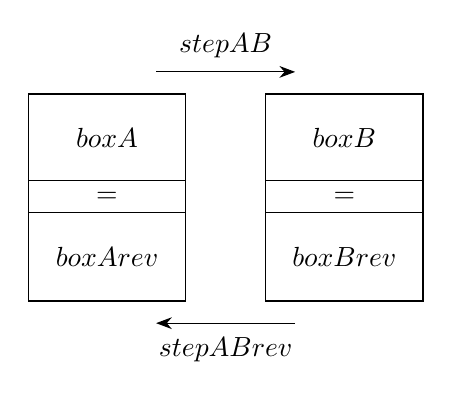
\begin{tikzpicture}
    \node[backtrack] (boxA) at (0, 0) {$\boxA$};
    \node[backtrack] (boxB) [right=1cm of boxA] {$\boxB$};

    \node[backtrackeq] (boxAeq) [below=-1pt of boxA] {$=$};
    \node[backtrackeq] (boxBeq) [below=-1pt of boxB] {$=$};

    \node[backtrack] (boxArev) [below=-1pt of boxAeq] {$\boxArev$};
    \node[backtrack] (boxBrev) [below=-1pt of boxBeq] {$\boxBrev$};
        
    \node (boxAr) at ([yshift=24pt,xshift=5mm]boxA) { };
    \node (boxBl) at ([yshift=24pt,xshift=-5mm]boxB) { };
    \draw [line width=0.4pt,-{Stealth[length=2mm]}] (boxAr)  --node[backtrackstep,above=3.0pt] {$\stepAB$} (boxBl);
    
    \node (boxBrevl) at ([yshift=-24pt,xshift=-5mm]boxBrev) { };
    \node (boxArevr) at ([yshift=-24pt,xshift=5mm]boxArev) { };
    \draw [line width=0.4pt,-{Stealth[length=2mm]}] (boxBrevl)  --node[backtrackstep,below=3.0pt] {$\stepABrev$} (boxArevr);
    
\end{tikzpicture}

\end{document}
